\chapter{Blockchain}
\label{blockchain}

In recent years the term ``blockchain" has become increasingly common: we can read it on daily newspapers, they talk about 
it on TV shows and it is an hot topic in industry. One of the most famous products based on this technology is Bitcoin, a 
cryptocurrency with a huge audience of about 2.9 to 5.8 Million active wallets \cite{BitcoinStatisticsCambridge} around the 
world.

The objective of this chapter is to introduce the reader in the blockchain technology describing its principles and features.

Section \ref{blockchain:overview} introduce the blockchain and its more important characteristics. Section 
\ref{blockchain:structure} presents the different components of the technology. Finally, section \ref{blockchain:ethereum} 
introduce Ethereum and section \ref{blockchain:ethereum_tools} shows some usefull tools to work with it.


\section{Overview on blockchain technology}
\label{blockchain:overview}
The blockchain is a set of techniques and protocols that allows the realization of a distributed ledger. In a blockchain 
system, the ledger is replicated in a large number of identical databases, each hosted and mantained by an interested party. 
When changes are entered in one copy, all the other copies are consequently updated. This database can be viewed as a public, 
secure distributed registry \cite{TruthAboutBlockchain}. It has some main characteristics following described:

\begin{itemize}
    \item \textbf{Decentralization}, this is one of the most important aspects of the blockchain: this technology doesn’t rely 
    on a central point of control which could be viewed as a single point of failure. This property makes the blockchain 
    fairer and considerably more secure. Consensus protocols are used across a network of nodes to validate and record data in 
    an incorruptible and accurate way.
    
    \item \textbf{Trasparecy}, data stored on the blockchain are public and every one can read them, usually using an Explorer, 
    that is a tool that shows them in an integrated way.

    \item \textbf{Security}, in fact the ownership of an address, and all the assets associated with it, is based on a strong 
    cryptography with public and private keys. This system prevent the risk of ``stolen identity" beacuse there is not a 
    direct connection between an address and an identity. Other aspects that increase the security are the Decentralization, 
    described before, and the blockchain structure that will be explained in next sections.

    \item \textbf{Immutability}, the information stored on the blockchain are really complex to corrupt thanks to the 
    decentralized nature of the system. To edit these data it needs that the majority of the nodes of the network (peers) agree 
    with the changes otherwise it will not take place. This capability also increase the security of the system because an 
    hacker cannot alter info resident on the blockchain, or more precisely, it is too expensive to do (even if theoretically 
    possible with an attack that add to the network a huge number of peer until reach the 51\% of controlled nodes).
    
    \item \textbf{Privacy}, blockchain also ensures the respect of the privacy of its users: a person is represented as an 
    address so no personal information (name, email, phone numbers) is exposed directly from the technology.
\end{itemize}

\section{Structure}
\label{blockchain:structure}

The term ``blockchain" is self-explanatory and it describe the logical structure of the technology: a chain of 
\textbf{blocks} where each block refers to the previous one. Inside every block there is a list of \textbf{Transactions}.

\begin{figure}[!ht]
    \centering
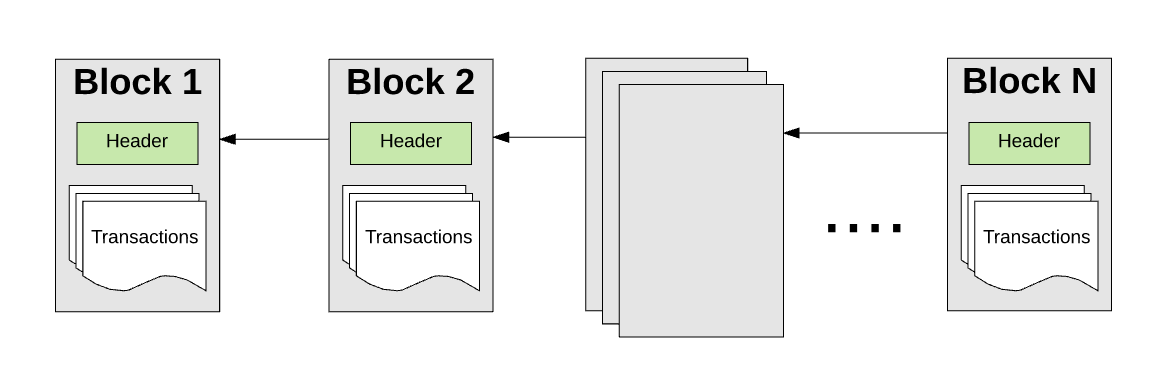
\includegraphics[width=\textwidth]{images/chain_of_blocks.png}
    \caption{Representation of a chain of blocks \cite{Medium}}
    \label{images:chain_of_blocks}
\end{figure}

Blocks are composed by an header and a body. The body simply contains the list of transactions associated with the block; the 
header instead contains general informations such as the hash of the current and of the previous block (in order to build a 
chain), the Merkle root that is an hash of the root of the Merkle tree in which are organized the transactions.
Apart these fundamentals properties every blockchain implementation can add its own header fields: common fields are nonce, 
the version of the system, the number of transactions contained etc.

Transactions are the minimal unit of information handled in the blockchain systems. Simply put, a transaction describes a 
transfer of information from an address to another. Every block can contains some hundreds of transactions.


\section{Ethereum}
\label{blockchain:ethereum}
All features and benefits described until now are common to all blockchain platforms but every product can 
add its own implementation over that or customize some behaviours.

One of the most famous and interesting platform available on the market today is \textbf{Ethereum}. It's 
an open source project, this means that everyone can contribute in his development and download its source 
code to understand in detail how it works.
\begin{figure}[!ht]
    \centering

\includegraphics[width=105mm]{images/ethereum.jpg}
    \caption{Ethereum project icon}
    \label{images:ethereum}
\end{figure}
Ethereum has a main peculiarity compared to its competitors: it was designed to be flexible and to adapt to 
different contexts, to be general-purpose.
In order to achive these objectives it is based on the \textbf{Ethereum Virtual Machine} (EVM) that is 
the ``runtime" of this platform. EVM is ``Turing complete", this means that it can execute code of arbitrary 
algorithmic complexity. Every node connected on the blockchain execute its own EVM allowing for the 
maintenance of the consensus over the network, even if has a huge computational cost and makes the entire 
system slower.

The foundamental task of the EVM is to execute \textbf{Smart Contracts}.
Just the smart contracts are the tools that allow Ethereum to be so flexible and generalized. Practically 
they are pieces of code that can do virtually everything, they reside on the blockchain and are loaded 
from users. This means that every user with a minimal programming background can partialy lead Ethereum 
behaviour.

The concept of ``Smart Contract" implicitly introduces the notion of \textbf{DAPP}: the DAPPs are common applications (web 
sites, mobile or desktop applications or also IoT apps) that uses as server the blockchain through the usage of a Smart 
Contract. In practice smart contracts are a middleware used to store data or execute actions on Ethereum. Actually there are 
a lot of DAPP in production on Ethereum and other in development but with some active users; they are about the most disparate 
business areas: there are a lot of games, a lot of cryptocurrencies and of exchanges, then some identity managers or food 
traceability. Figure \ref{images:solution_architecture} shows an example of an architecture of a system based on Ethereum.

\begin{figure}[!ht]
    \centering
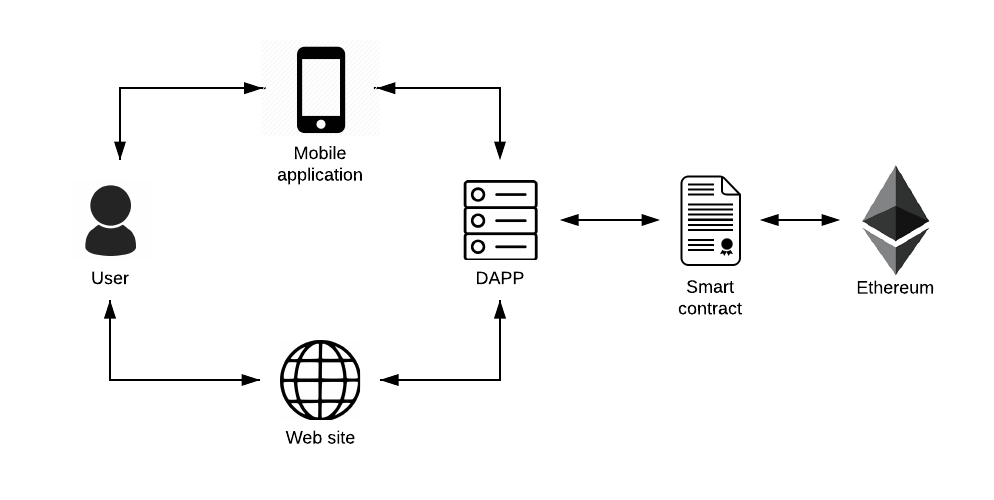
\includegraphics[width=\textwidth]{images/solution_architecture.png}
    \caption{Example of a solution architecture}
    \label{images:solution_architecture}
\end{figure}

Every operation executed by the EVM (storage of information, contract execution and so on) has a cost: for every transaction 
users must pay a small fees to the network. This payment has two main advantages: it prevents malicious computational tasks 
(DDoS attacks) and encourages people to mine Ethereum. The mining is the process of receive, propagate, verify, execute 
transactions and group them in blocks. These tasks are complex and really expensive from the computational point of view for 
this powerfull hardware and good electrical system are needed to do that. Miners are rewared for each block they mine with 
\textbf{Ether} (ETH), Ethereum’s native value-token.

Addresses in Ethereum are called \textbf{Accounts} and there are two kind of them: Externally Owned Accounts (EOAs) that are 
accounts handled by a person or an organization of the real world and Smart Contracts.

Ethereum transactions, over the fields common to all blockchain technologies, have a set of peculiar properties. Figure 
\ref{images:transactions_structure} is a screenshot taken from Etherscan (\ref{blockchain:ethereum_tools}) and shows the 
structure of a transaction in Ethereum. It has these properties:

\begin{itemize}
    \item \textbf{TxHash}, is the hash of the transaction, a way to uniquely identify it
    \item \textbf{Block Height}, is a reference to the block that contains the transaction (using its index)
    \item \textbf{Timestamp}, indicates when the transaction has been added to the blockchain
    \item \textbf{From}, represents the address from which the transaction start (the sender)
    \item \textbf{To}, is the address to which the transaction arrive (the receiver)
    \item \textbf{Value}, reveals the amount of Ether exchanged in the transaction
    \item \textbf{Gas limit}, shows the limit of gas that can be spend in a single transaction
    \item \textbf{Gas Used By Transaction}, defines the effectively used amount of gas (less then or equal to Gas Limit)
    \item \textbf{Gas Price}, is the price of the single unit of gas
    \item \textbf{Actual Tx Cost/Fee}, indicates the cost of the mining of the transaction (Gas price * Gas used)
    \item \textbf{Nonce}, is a value that enable to satisfy the proof-of-work
\end{itemize}

In general apart from the presented fields there is another one in Ethereum transactions: the ``Input Data" used to pass 
parameters or, for contracts, to select which method to execute.

\begin{figure}[!ht]
    \centering
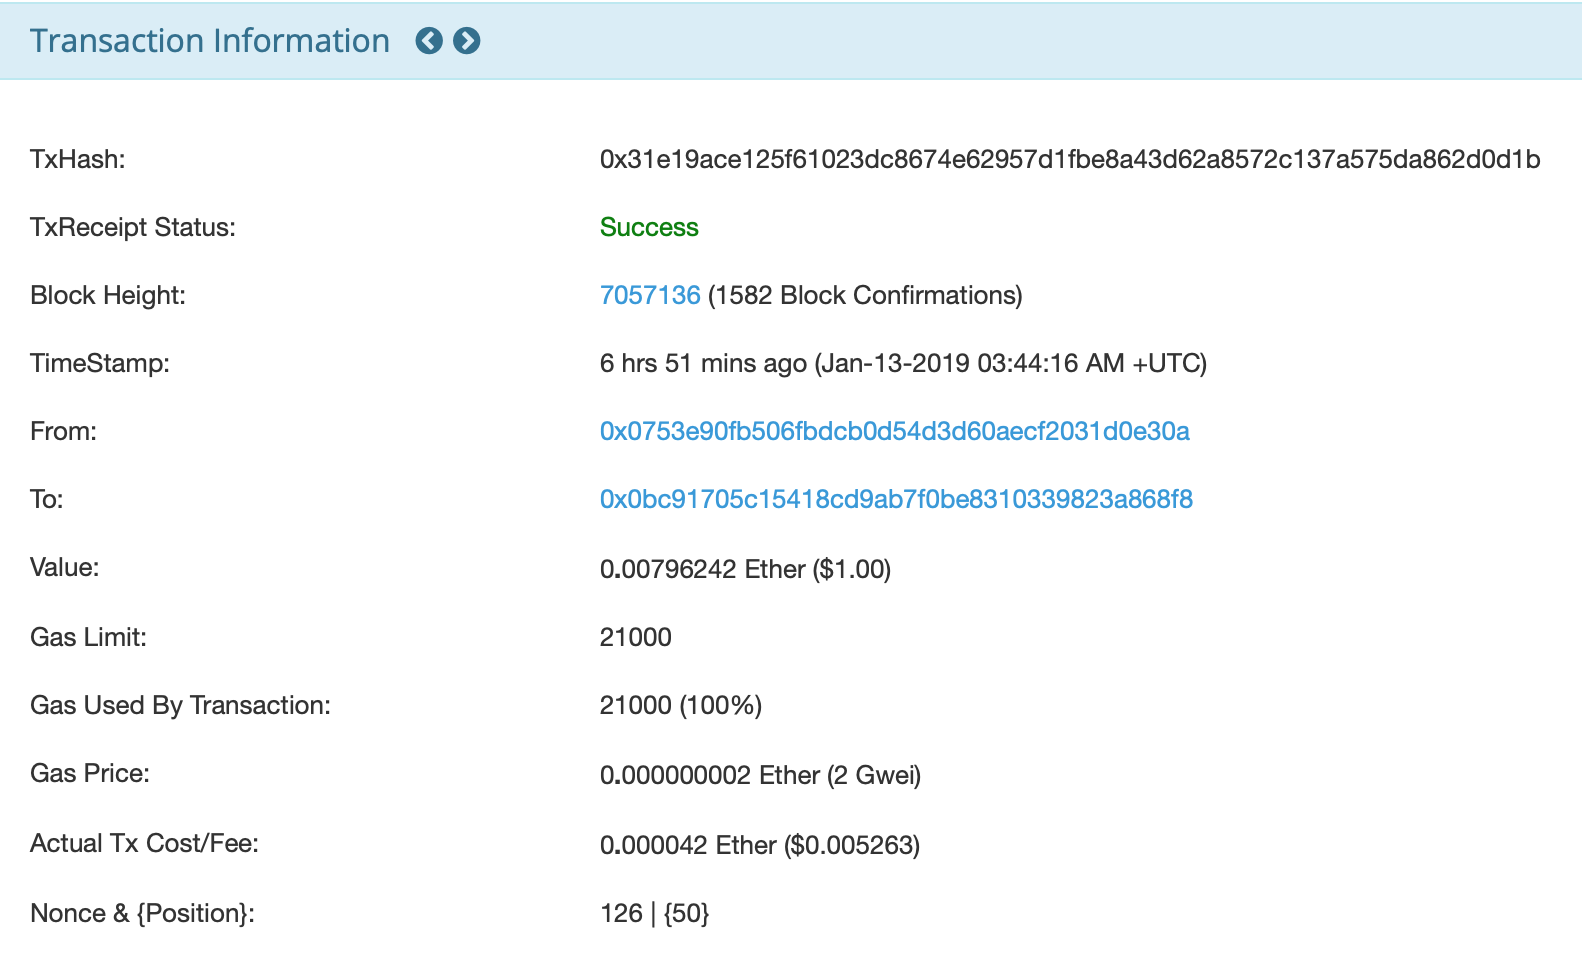
\includegraphics[width=\textwidth]{images/transactions_structure.png}
    \caption{Structure of an Ethereum transaction}
    \label{images:transactions_structure}
\end{figure}



\section{Ethereum tools}
\label{blockchain:ethereum_tools}
In order to work with Ethereum there are some tools needed and other that makes your life simpler.

\subsection{Clients}
Everyone can build its own Ethereum node with few simple steps: it is enough to install a client on a machine. There are a lot 
of official clients developed in various programming languages and that support almost all operating systems. Every client 
has its advantages and disadvantages even if all of them are pretty stable; the most used clients are \textbf{Parity}, 
\textbf{Go-Ethereum} and \textbf{Cpp-Ethereum}. After the installation these applications start the syncronization to the 
network: this is a costly operation that can take from various hours up to few days and will occupy some tens of GB on the 
machine disk. A local node can be referred in order to execute transactions, load contracts and interact in any other way with 
the blockchain.

\subsection{Explorers}
To read data from Ethereum there are different possible approaches: usually clients offer a UI and sometimes there are sections 
to explore data stored in the blockchain. Another chance consist in using the api exposed from the clients (RPC calls) to 
obtain row data. Anyway none of these two approaches are so comfortable: the first one allows to access only a subset of the 
data and the second one imply a certain technical competence. In general Explorer are used. Explorers are softwares that 
indexes all data on the blockchain in order to have a fast access to them. The most famous and used Etehreum explorer is 
Etherscan (https://etherscan.io). Etherscan allows the user to access all data on Ethereum in a very rapid way, its dataset is 
updated on the fly and shows some summary charts. Morover it expose some APIs for registered users that helps developers to 
get blockchain data in an aggregate form.

\subsection{Solidity}
Developers who wants to develop a Smart Contract should study \textbf{Solidy}. Solidity is a Contract-Oriented programming 
language influenced by C++, Python and JavaScript and is designed to target the EVM. Solidity is statically typed, supports 
inheritance, libraries and complex user-defined types among other features.

Listing \ref{listing:solidity} shows a very simple example of Smart Contract that allows users to store a numeric value on 
the blockchain.

\begin{lstlisting} [caption = {Simple solidity contract}, label = {listing:solidity}, language=Solidity]
    pragma solidity ^0.5.0;

    contract SimpleStorage {
        uint storedData;

        function set(uint x) public {
            storedData = x;
        }

        function get() public view returns (uint) {
            return storedData;
        }
    }
\end{lstlisting}

In general solidity supports classical value types such as boolean, integers and strings but it also supports a value type 
called ``address": it is a reference to an Ethereum address that can be used to Ether exchanges. All common  control-flow 
expressions are supported (if, else, while, return, etc.) Also visibility constructs are available: external, public, internal 
and private: every of them decide if a function or a property is available to the outside of the contract and/or to its 
internal.

Solidity supports multiple inheritance including polymorphism. When a contract inherits from other contracts, only a single 
contract is created on the blockchain, and the code from all the base contracts is compiled into the created contract. 
Another important tool for solidity developers are interfaces: they are similar to abstract contracts, but they cannot have 
any functions implemented. There are further restrictions:

\begin{itemize}
    \item They cannot inherit other contracts or interfaces.
    \item All declared functions must be external.
    \item They cannot declare a constructor.
    \item They cannot declare state variables.
\end{itemize}

Often interfaces are used to join to some standard as for example ERC20 tokens.


\subsection{Web3.js}
Last but not least tool introduced is Web3.js. This is a javascript library that exposes some incredibly simple apis that 
allow developers to interact with the blockchain. In practice this library interacts with a network node (local or remote, it 
does not matter) calling the RPC exposed from some client installed into the node address. 
Practically this library act as a gateway, hiding the complexity of an RPC call to the developer that simply invoke a 
javascript function. Then the client does his work and returns results to Web3.js which in its turn forward these results to 
the caller javascript application.

This library has a lot of features: it allows to reading the data on the blockchain, to register for Ethereum events (as for example 
new blocks or transactions), to invoke contracts and to manage personal informations and wallets.